\documentclass[tikz,border=2pt]{standalone}
\usepackage{amsmath,amssymb}
\usepackage{tikz}
\usetikzlibrary{arrows.meta}

\begin{document}
% Residual capacities for one edge: with capacity 4 and current flow 3, one more unit can go
% forward and 3 units can be cancelled backward; the residual network collects these.
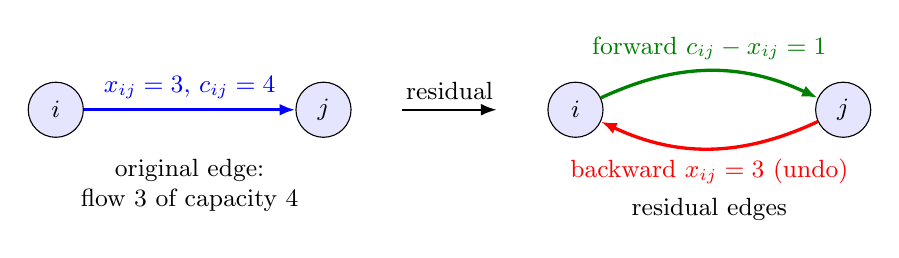
\begin{tikzpicture}[every node/.style={font=\small}, >={Latex[length=2mm]}, v/.style={draw, circle, fill=blue!10, minimum size=7mm, inner sep=0pt}]
	\begin{scope}
		\node[v] (i) at (0,0) {$i$}; \node[v] (j) at (3.4,0) {$j$};
		\draw[->, very thick, blue] (i) -- (j) node[midway, above, font=\small] {$x_{ij}=3$, $c_{ij}=4$};
		\node[anchor=north, font=\small, align=center] at (1.7,-0.5) {original edge:\\ flow $3$ of capacity $4$};
	\end{scope}
	\draw[->, thick] (4.4,0) -- (5.6,0) node[midway, above, font=\small] {residual};
	\begin{scope}[xshift=6.6cm]
		\node[v] (i) at (0,0) {$i$}; \node[v] (j) at (3.4,0) {$j$};
		\draw[->, very thick, green!50!black] (i) to[bend left=25] node[midway, above, font=\small] {forward $c_{ij}-x_{ij}=1$} (j);
		\draw[->, very thick, red] (j) to[bend left=25] node[midway, below, font=\small] {backward $x_{ij}=3$ (undo)} (i);
		\node[anchor=north, font=\small] at (1.7,-1.0) {residual edges};
	\end{scope}
	\end{tikzpicture}
\end{document}
